\documentclass[conference,compsoc]{IEEEtran}
\usepackage{cite}
\usepackage[english]{babel}
\usepackage[pdftex]{graphicx}
 \usepackage{array}
\usepackage{multirow}
\DeclareGraphicsExtensions{.pdf,.jpeg,.png}
\usepackage{amsmath}
\usepackage{hyperref}
\usepackage[caption=false,font=footnotesize,labelfont=sf,textfont=sf]{subfig}
\usepackage{url}
\hyphenation{op-tical net-works semi-conduc-tor}

\makeatletter
\def\endthebibliography{%
	\def\@noitemerr{\@latex@warning{Empty `thebibliography' environment}}%
	\endlist
}
\makeatother

\begin{document}
\title{Data Driven Project Management: \\ Predicting the Development Time}


\author{\IEEEauthorblockN{Marko Prelevikj}
	\IEEEauthorblockA{Faculty of Computer and Information Science\\
		University of Ljubljana\\
		Ljubljana, Slovenia\\
		Email: mp2638@stuent.uni-lj.si}
}

\maketitle

\begin{abstract}
%Predicting development time is hard. In this paper we are trying to explain all the difficulties encountered on the journey to predicting time with as low 

\end{abstract}

\IEEEpeerreviewmaketitle

\section{Introduction}

%Project managers are faced with time estimation on a daily basis.
The project manager's (PM) main task is to break down the project they manage into tasks which are manageable, not very complex and make a round unit which can be executed with the knowledge of a single person.
Once the project is broken down into pieces the PM needs to answer the following questions for each task:
\begin{enumerate}
	\item how much time the task is going to take to develop; and
	\item which project member is the best fit for the task
\end{enumerate}
% ^ can be omitted if needed
In this paper we are focusing on the task of estimating the time required to develop a given task. We use data provided from a company's JIRA portal~\cite{JIRA}, which keeps record of the project's tasks. We made 4 different models of the time required to develop a task, where we changed the unit we are forecasting in: days or hours, and the time span of development time, ranging from all time down to a maximum of 10 days. We evaluated the variations of the model using 4 distinct methods: Naive Bayes, Random Forests, XGBoost~\cite{chen2016xgboost} and SVM. In the end we uncover which are the most important features of the task which should be considered when estimating the development time for which we used the SHAP~\cite{lundberg2020local2global} method.

%In this paper, we are addressing the problem of time estimation because it is very often that PMs do know who to assign the tasks to, based on project member's skill set, availability and other information that is not tracked by any software, which makes the problem much more difficult to address. On the other hand, time estimation is a problem which can be addressed because PMs keep record of all the tasks which can be processed. 
%With some preprocessing of the available historical task information we were able to build a model of the time required to develop a task. Along the way we 

%Project managers (PMs) need to assess each piece of the project they manage so they can delegate the pieces to the rest of the project members to be executed. The project pieces can be referred to with multiple terms, such as tasks, tickets, issues; and we are going to use these terms interchangeably. The task is a unit which (generally) cannot be broken down into subunits and it should be addressed as a whole. 

\section{Model data}
The available information used to build the model has been extracted from a company's JIRA portal~\cite{JIRA}. All tasks are described by their categorical features: \textit{type}, \textit{priority}, \textit{components} of the project they affect, and \textit{labels} which are specific for the project. Due to their high cardinality, the values of the \textit{components} and \textit{labels} features have been filtered such that there are only left values which have at least 50 entries in the dataset. The filtered values are used in their one-hot-encoded form to reduce the complexity of the model. Additionally, we used the following discrete features: the \textit{number of comments} each task has, the \textit{number of linked issues}, and their \textit{degree of cycling}.

% noise reduction
Due to improper usage of JIRA, there is some noise in the data, which causes a strong bias toward low values of the predicted time to develop. To reduce this effect we have filtered out all tasks which have development time lower than $2h$. To further reduce the variance in our dataset we have decided to limit the upper bound of the development time. We have done so in 3 different stages to measure the effect of the variance on our model: 1) there is no upper bound, 2) the upper bound is 30 days, and 3) the upper bound is 10 days. The summary of the datasets is shown in Table~\ref{dataset_description}.

% model features, TODO: write about real vs ideal model, why we omit #comments and degreeOfCycling




\section{Testing model quality}
Present different the results (MAE, RMSE, R2) obtained by different regressors.
As the variance lowers, so do the metrics of quality of the models.

\section{Model Explainability}
Write about feature importance and how to explain the made decisions.


\section{Conclusion}
Quick recap of the problem and how we solved it.
XGBoost~\cite{chen2016xgboost}, SHAP~\cite{lundberg2020local2global}.

\begin{figure}[!t]
\centering
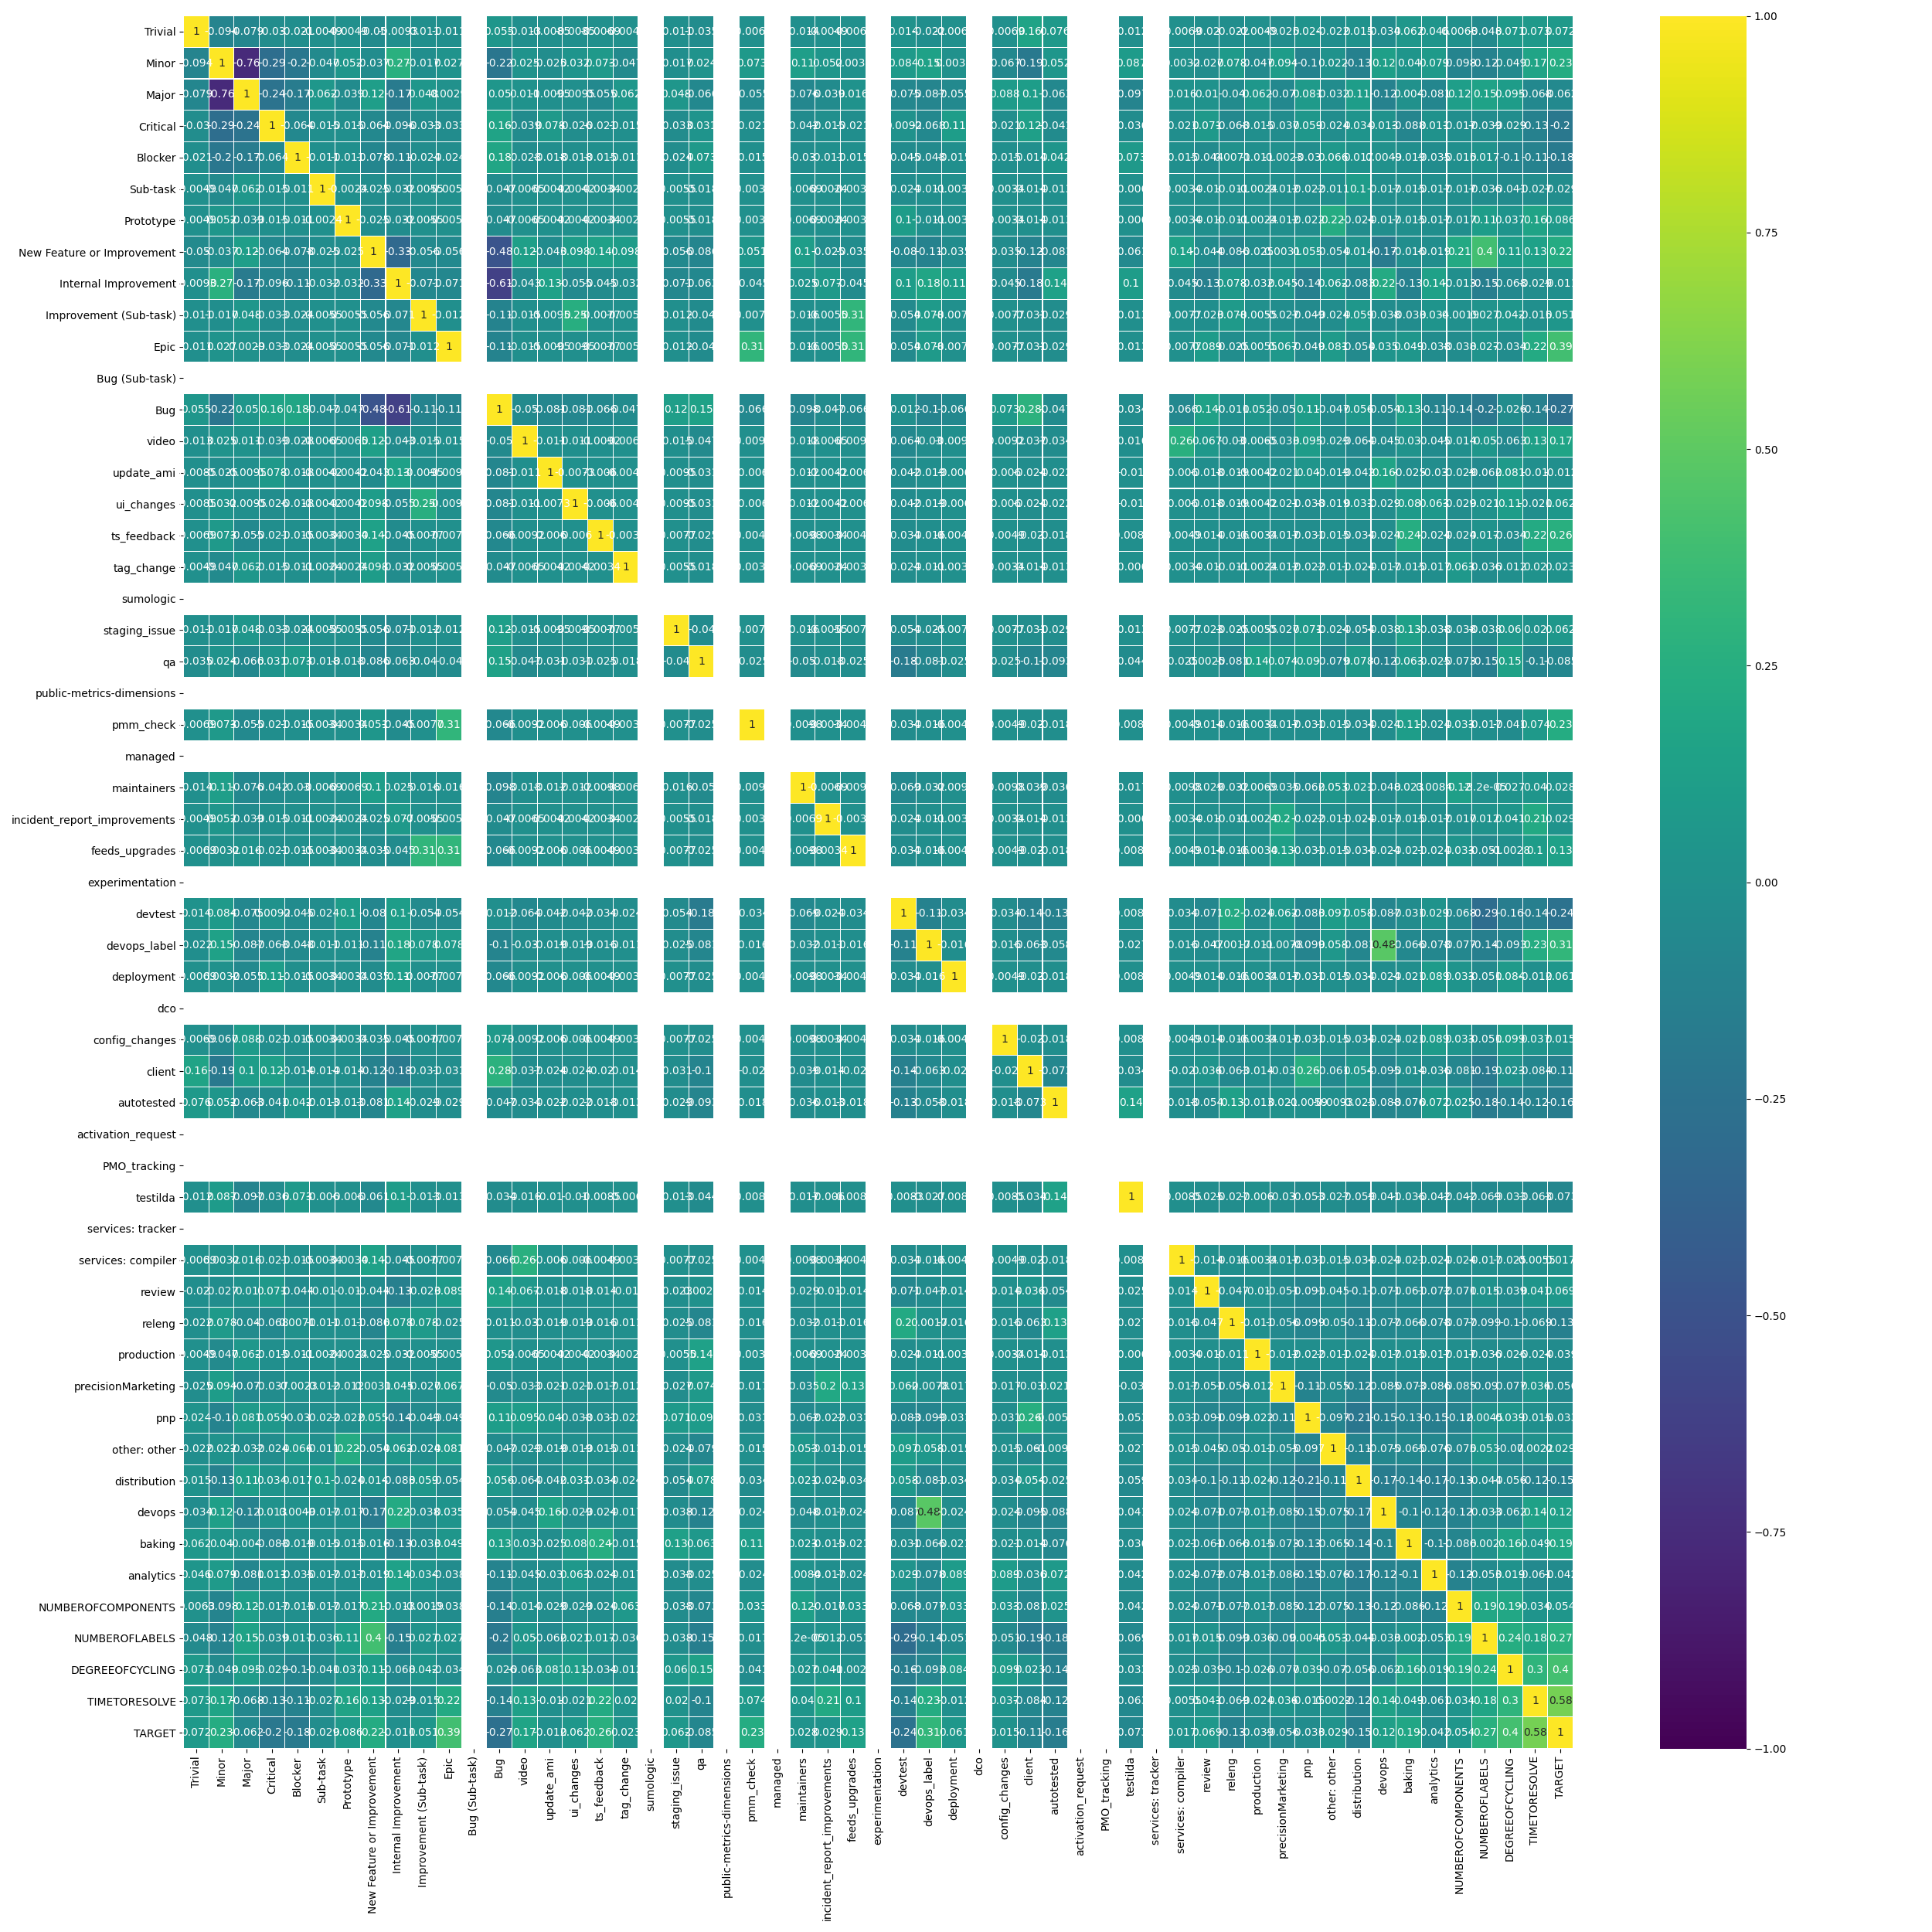
\includegraphics[width=2.5in]{feature_correlation.png}
\caption{Simulation results for the network.}
\label{fig_sim}
\end{figure}

\begin{figure*}[!t]
\centering
\subfloat[Case I]{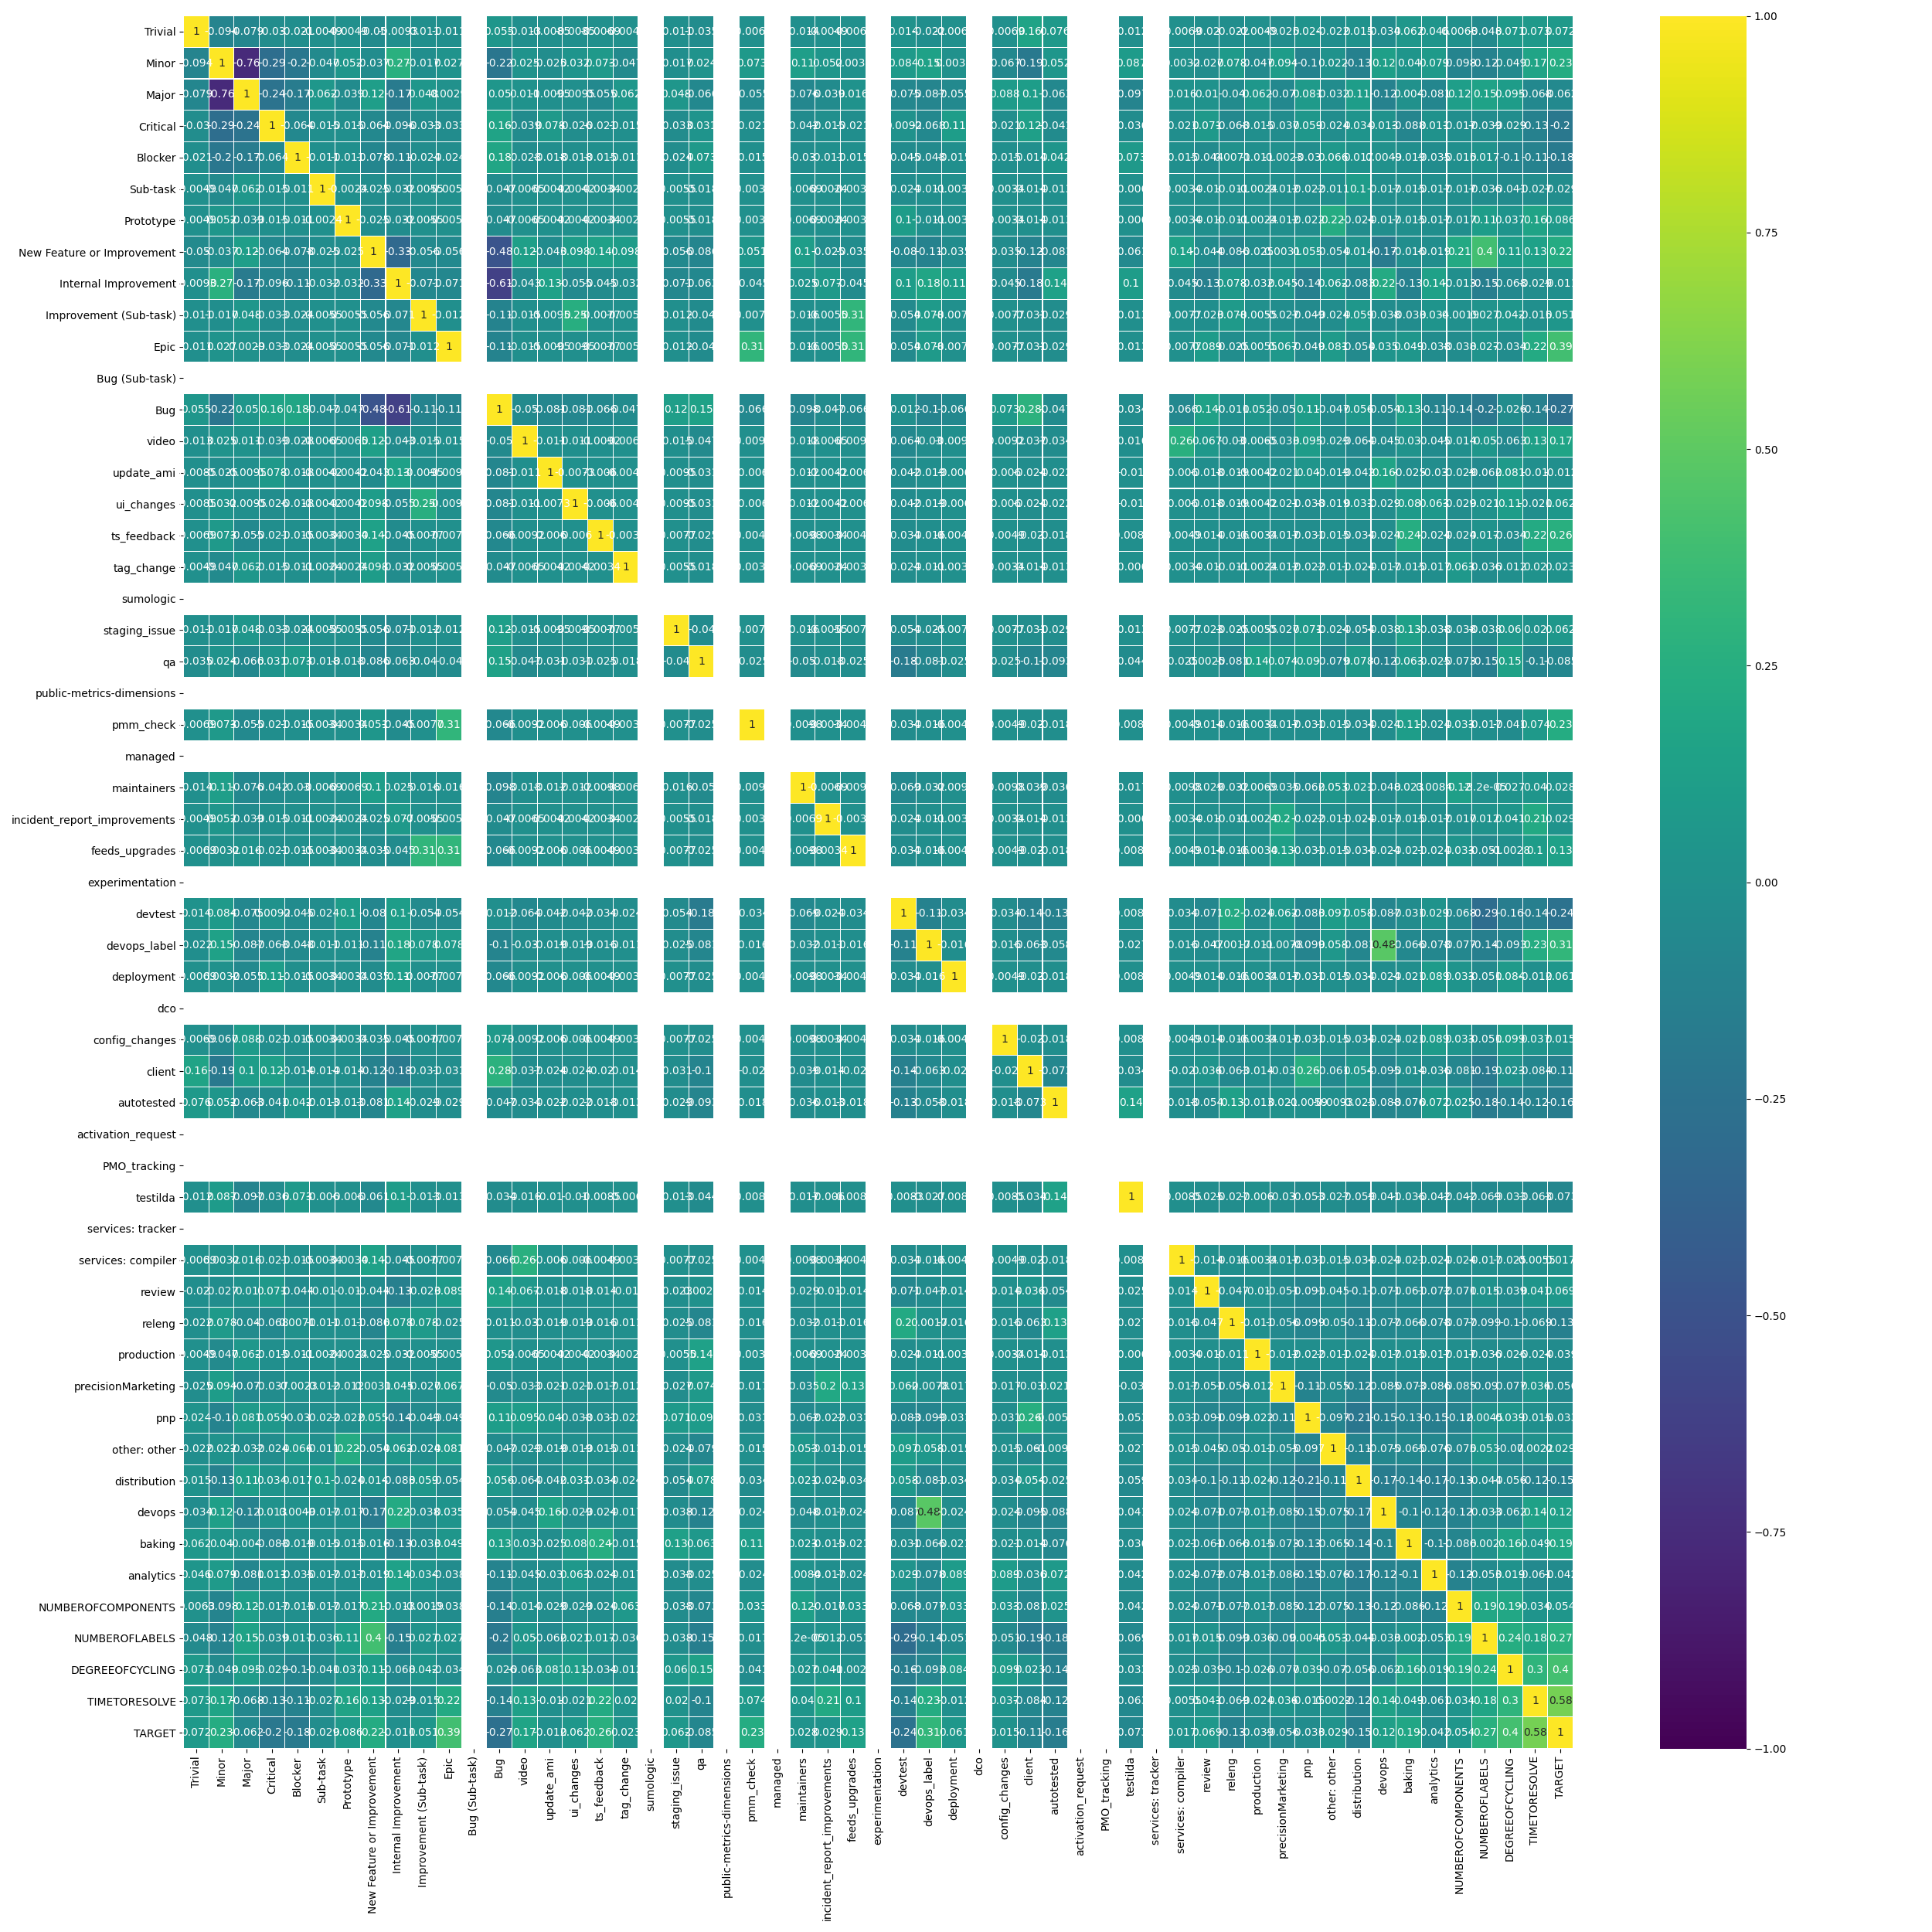
\includegraphics[width=2.5in]{feature_correlation.png}%
\label{fig_first_case}}
\hfil
\subfloat[Case II]{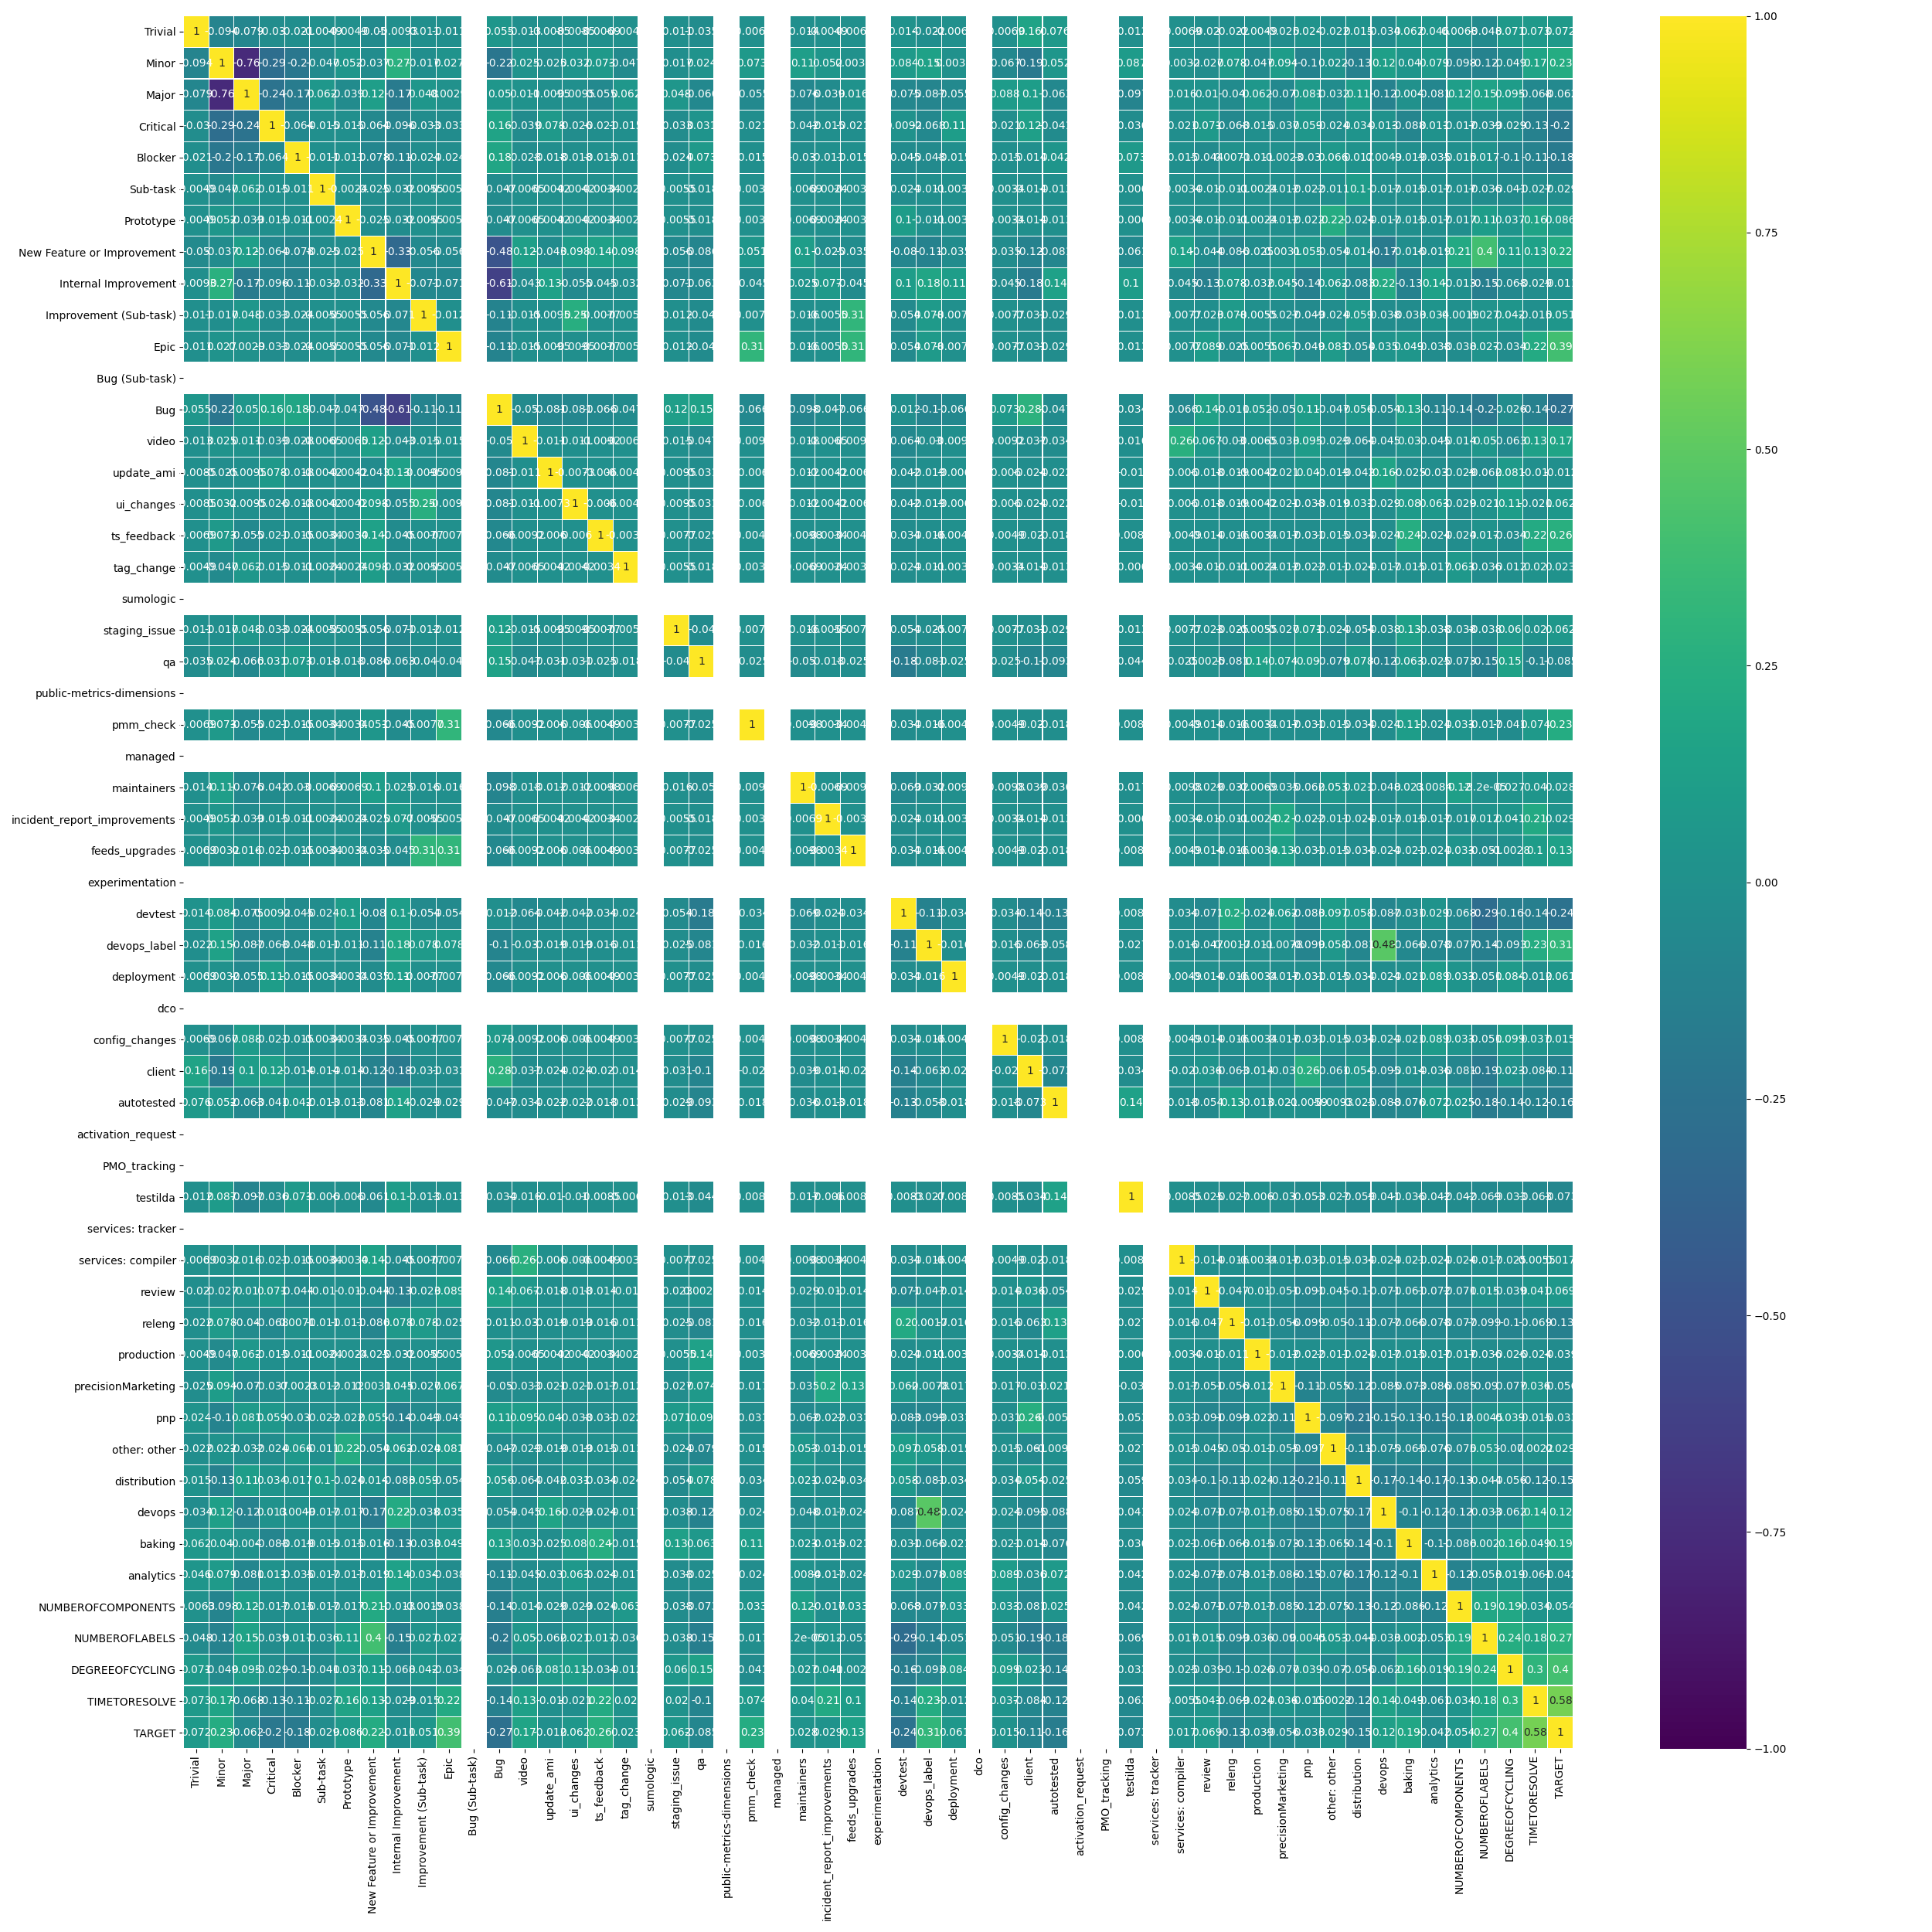
\includegraphics[width=2.5in]{feature_correlation.png}%
\label{fig_second_case}}
\caption{Simulation results for the network.}
\label{fig_sim2}
\end{figure*}

\begin{table}[!t]
	\renewcommand{\arraystretch}{1.3}
	\caption{Dataset characteristics. }
	\label{dataset_description}
	\centering
	\begin{tabular}{c|r|r|r|r}
		Statistic &        All  & 1 Q & 1 M & 10 D \\
		\hline
		count &  2935.000  &     2902.000  &   2775.000 &   2451.000 \\
		mean  &   205.252  &      149.210  &     96.165 &     55.762 \\
		std   &   678.103  &      293.573  &    132.257 &     57.019 \\
		min   &     2.000  &        2.000  &      2.000 &      2.000 \\
		25\%   &    15.000  &       15.000  &     13.000 &     11.000 \\
		50\%   &    49.000  &       48.000  &     44.000 &     33.000 \\
		75\%   &   148.000  &      143.000  &    121.000 &     83.000 \\
		max   & 15003.000  &     2260.000  &    754.000 &    228.000 \\

	\end{tabular}
\end{table}

\begin{table}[!t]
	
	\renewcommand{\arraystretch}{1.3}
	\label{model_performance}
	\centering
	\caption{Performance of different methods on the variations of the dataset. The $*$ symbol indicates that the dataset does not contain all the initial attributes, thus it is more realistic.}
	\begin{tabular}{c|c|c|c|c}
		DataSet & Method & RMSE & MAE & $R^2$ \\
%		\hline
%		\multirow{4}{*}{All}
%		& boost & 807.362 & 279.128 & -0.085 \\
%		& naive & 896.482 & 387.358 & -0.337 \\
%		& forest & 1028.401 & 286.985 & -0.760 \\
%		& SVM & \textbf{792.794} & \textbf{192.552} & -0.046 \\
		\hline
		\multirow{4}{*}{All*}
		& boost & \textbf{791.428} & 254.770 & -0.042 \\
		& naive & 948.649 & 420.036 & -0.498 \\
		& forest & 840.027 & 256.399 & -0.174 \\
		& SVM & 792.344 & \textbf{191.267} & -0.045 \\
%		\hline
%		\multirow{4}{*}{1Q}
%		& boost & \textbf{282.812} & 161.298 & 0.045 \\
%		& naive & 521.056 & 340.146 & -2.242 \\
%		& forest & 339.457 & 165.115 & -0.376 \\
%		& SVM & 303.855 & \textbf{125.127} & -0.102 \\
		\hline
		\multirow{4}{*}{1Q*}
		& boost & \textbf{286.835} & 160.587 & 0.018 \\
		& naive & 577.520 & 389.602 & -2.982 \\
		& forest & 361.223 & 179.258 & -0.558 \\
		& SVM & 302.772 & \textbf{124.272} & -0.095 \\
%		\hline
%		\multirow{4}{*}{1M}
%		& boost & \textbf{139.968} & 95.641 & -0.078 \\
%		& naive & 242.789 & 202.094 & -2.242 \\
%		& forest & 181.735 & 110.973 & -0.817 \\
%		& SVM & 144.071 & \textbf{78.272} & -0.142 \\
		\hline
		\multirow{4}{*}{1M*}
		& boost & \textbf{138.034} & 92.616 & -0.048 \\
		& naive & 255.083 & 213.834 & -2.579 \\
		& forest & 178.280 & 109.402 & -0.748 \\
		& SVM & 143.368 & \textbf{78.249} & -0.131 \\
%		\hline
%		\multirow{4}{*}{10D}
%		& boost & \textbf{56.809} & 44.098 & 0.028 \\
%		& naive & 112.730 & 99.071 & -2.828 \\
%		& forest & 74.592 & 53.483 & -0.676 \\
%		& SVM & 61.194 & 42.053 & -0.128 \\
		\hline
		\multirow{4}{*}{10D*}
		& boost & \textbf{56.406} & 43.847 & 0.041 \\
		& naive & 120.824 & 106.642 & -3.398 \\
		& forest & 77.243 & 56.629 & -0.797 \\
		& SVM & 60.460 & \textbf{41.976} & -0.101 \\
	\end{tabular}
\end{table}

\bibliographystyle{IEEEtran}
\bibliography{./references}
\end{document}


